\chapter{Graph Visualization}
Gvis is designed to be intuitive and easy to use. It is implemented in java swing and uses the graphstream library \cite{graphstream} for the underlying graph visualization and layouting. Figure \ref{ex:ui-full} shows an example gvis window.

\begin{figure} [h]
\centering
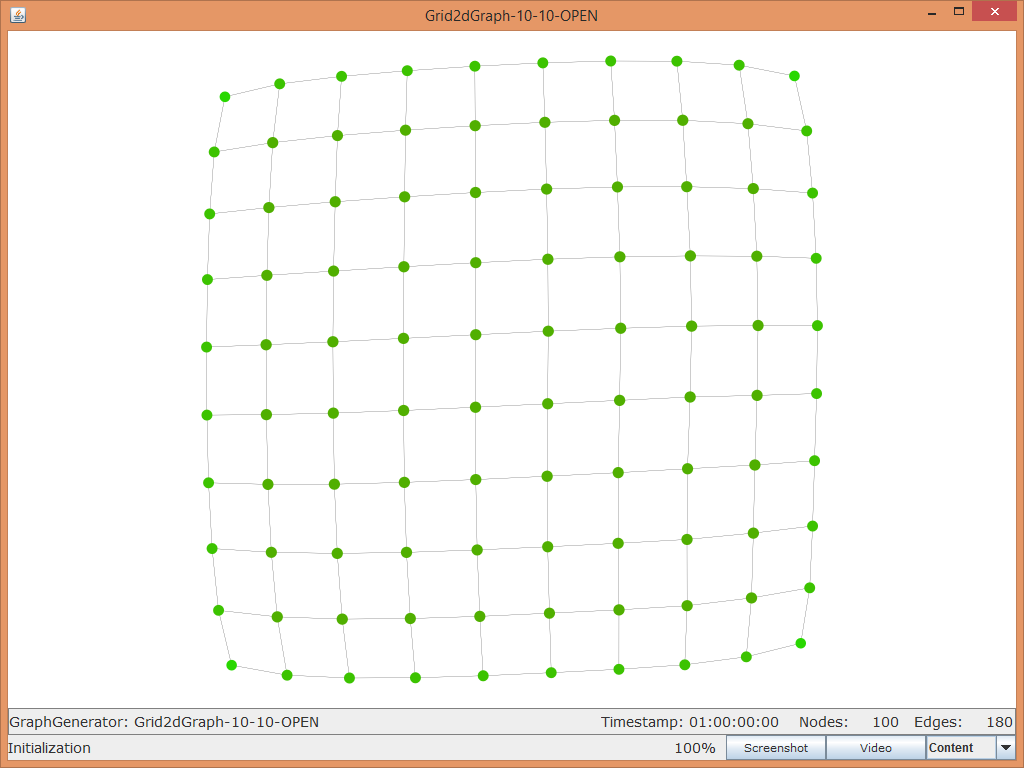
\includegraphics [scale=0.45] {images/ui-full}
\caption{Example of the graph visualization interface.}
\label{ex:ui-full}
\end{figure}

\section{Interface}
\label{s:interface}
The interface is divided into two different areas, the graph area and the information area, see \ref{ex:ui-areas}. The graph area displays the graph and allows some user interaction, for example dragging nodes, zooming with the mousewheel or moving in the graph with right mouse button pressed. The information area consists of the StatPanel, which shows basic information, and the TextPanel, which shows a status text and allows the user to capture screenshots or videos of the gvis window, see \ref{ex:ui-information}. The capture area selection shows what parts of the window will be captured with screenshots or videos. Selecting \emph{graph} will only capture the graph area. \emph{Content} will capture graph and information area. \emph{Full} will capture the entire window including its border. Note that recordings require the window to stay visible and at the same position.

\begin{figure} [h]
\centering
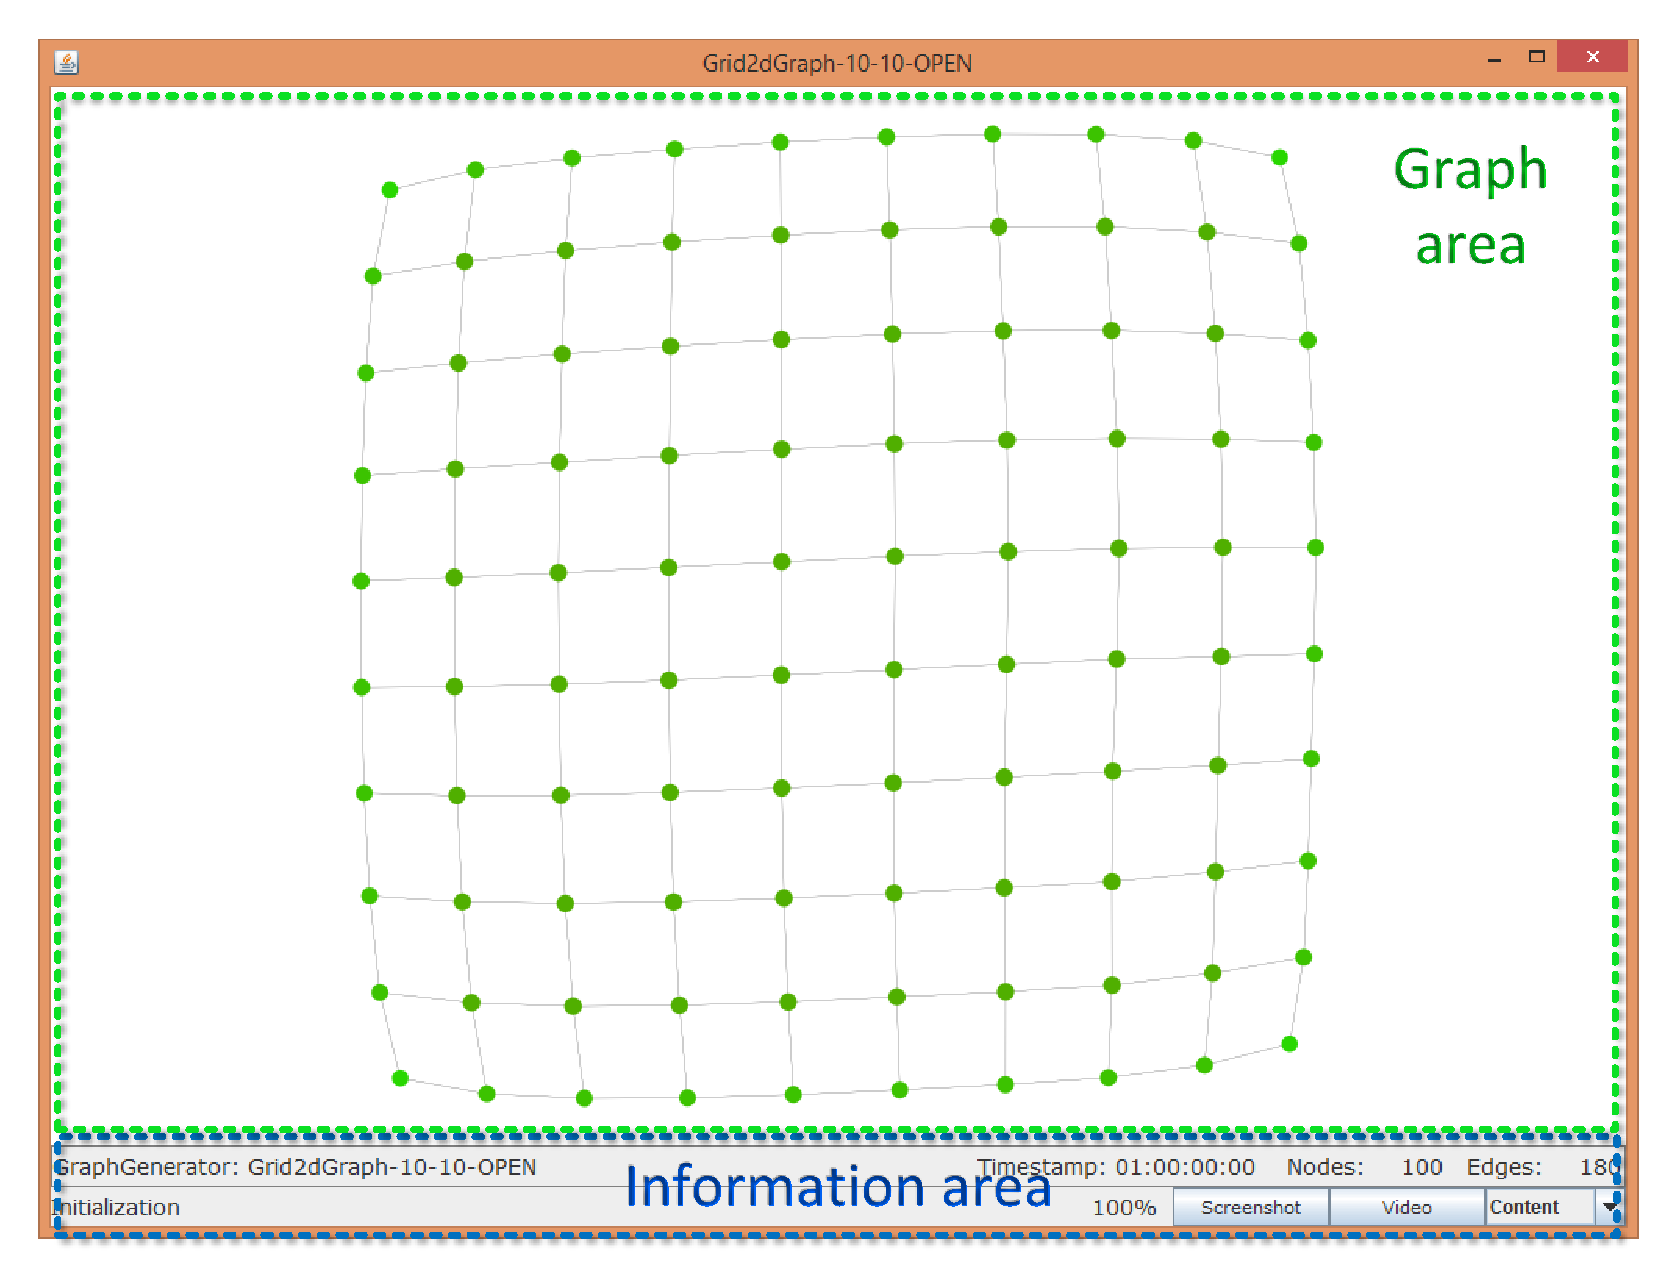
\includegraphics [scale=0.45] {images/ui-areas.pdf}
\caption{Different interface areas.}
\label{ex:ui-areas}
\end{figure}
\begin{figure} [h]
\centering
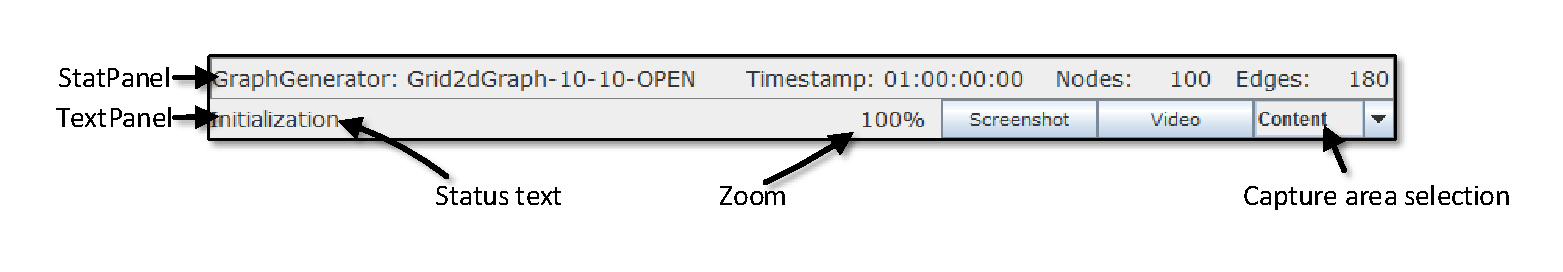
\includegraphics [scale=0.6] {images/ui-information.pdf}
\caption{The information area.}
\label{ex:ui-information}
\end{figure}


\subsection{ToolTips}
\label{ss:toolTips}
ToolTips are a special part of the graph visualization. They reveal additional information to the user and offer basic interactions with the underlying graph. Each node in the graph may have its own ToolTips, which can be shown and hidden by clicking the node with the right mouse-button. Figure \ref{fig:ToolTip} illustrates how the default ToolTips look like. Four ToolTips are visible: 
\begin{enumerate}
\item NodeIdLabel: Shows the node id.
\item NodeDegreeLabel: Shows the nodes degree.
\item FreezeButton: May be clicked to toggle freeze-mode on the node. This will (mostly) prevent the node to be moved during layouting and dragging of adjacent nodes.
\item HighlightButton: May be clicked several times to highlight the node, increasing its size.
\end{enumerate}
These ToolTips build the basic and default ToolTips to be used in gvis. However, the implementation of customized ToolTips is easy and will be discussed in section \ref{s:impl-tooltips}. How to enable ToolTips using the GraphVisConfig will be explained in section \ref{ss:toolTipsConfig}.

\begin{figure} [h]
\centering
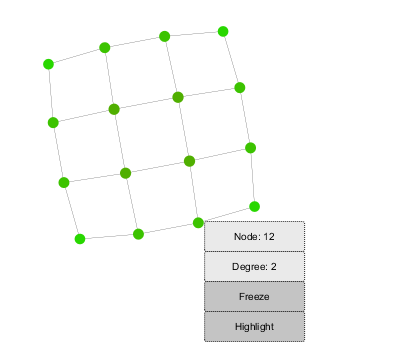
\includegraphics [scale=0.85] {images/tooltip}
\caption{Example of the default ToolTips.}
\label{fig:ToolTip}
\end{figure}

\section{Getting started}
\label{s:start}
Using the graph visualization part of DNA is very simple. It can be enabled/disabled with:
\begin{lstlisting}
	GraphVisualization.enable();
	
	GraphVisualization.disable();
\end{lstlisting}
When the visualization is enabled it is sufficient to generate a graph using DNA. The visualization window will be initialized automatically and all events, like node or edge additions, occuring in the graph will be visualized. Figure \ref{code:gridGraph} shows a simple example resulting in a 2d grid-graph as shown in figure \ref{ex:ui-full}. For more details about graph generation in DNA check the generation documentation.

\begin{figure} [h]
\begin{lstlisting}
public static void main(String[] args) throws
				MetricNotApplicableException {
	// enable gvis
	GraphVisualization.enable();
			
	// init series
	GraphGenerator gg = new Grid2dGraph(GDS.undirected(), 10, 10,
			ClosedType.OPEN);
	BatchGenerator bg = new RandomBatch(5, 0, 10, 0);
	Series s = new Series(gg, bg, new Metric[0], "data/gvis-test/",
			"grid2dgraph");
				
	// generate
	SeriesData sd = s.generate(1, 0, false);
}

\end{lstlisting}
\caption{Example of visualizing a 2d GridGraph.}
\label{code:gridGraph}
\end{figure}